\documentclass[12pt]{article}

\usepackage{amsmath}
\usepackage{float}
\usepackage[margin=1.2in]{geometry}
\usepackage{listings}
\usepackage{color}
\usepackage{graphicx}
\usepackage{caption}
\usepackage{newfloat}
\usepackage{subcaption}
\usepackage{amssymb}
\usepackage{url}


\bibliography{ref}

\DeclareCaptionType{snip}[Typename][List of snippet]
\newenvironment{snippet}{\captionsetup{type=snippet}}{}


\DeclareFloatingEnvironment{Snippet}
\title{\bfseries Sorting Algorithms}
\author{Benjamin Hough, Erick Sanchez}
\date{May 18, 2016}

\usepackage{array}
\setlength\extrarowheight{3pt} 


\lstset{
	language=[Visual]C++,
	basicstyle=\footnotesize, 
	keywordstyle=\bfseries\ttfamily\color[rgb]{0,0,1},
	identifierstyle=\ttfamily,
	commentstyle=\color[rgb]{0.133,0.545,0.133},
	stringstyle=\ttfamily\color[rgb]{0.627,0.126,0.941},
	showstringspaces=false,
	numberstyle=\footnotesize,
	numbers=left,
	stepnumber=1,
	numbersep=10pt,
	tabsize=2,
	breaklines=true,
	prebreak = \raisebox{0ex}[0ex][0ex]{\ensuremath{\hookleftarrow}},
	breakatwhitespace=false,
	aboveskip={1.5\baselineskip},
	columns=fixed,
	extendedchars=true
	% frame=single,
	% backgroundcolor=\color{lbcolor},
}


\begin{document}
	
	\maketitle
	\section*{Abstract}
	
	In this paper we introduce algorithm efficiency with emphasis on sorting algorithms. 
	We discuss the two broad types of sorting algorithms, comparison and non-comparison, giving examples of each. 
	We explore a new version of merge sort written by us and do a detailed analysis of its performance compared to other mainstream algorithms. 
	We find that sorting efficiency is highly dependent on the data being sorted and going strictly by the given runtime approximation is not enough to guarantee maximum efficiency. 
	\newline
	\tableofcontents
	
	\pagebreak
	
	\section{Introduction} %"Introduction - Give a short but informative introduction to your chosen topic, including the current “state of the field” as appropriateOutline what you will do in the balance of the paper (ie. Explain the goals of the paper). Indicate why this topic is exciting/useful."
	
	 Sorting algorithms are a fundamental type of algorithm that many other more sophisticated algorithms are built upon\cite[p.~6]{intro}.
	 In the most abstract form, sorting algorithms take in a list of unordered items and output or modify the list to the desired order, whatever it may be$~\footnote{typically numeric or alphabetic order is used}$.
	 The goal of our research was to gain a better understanding of sorting algorithms in general and to learn the nuances between the different types of algorithms available.
	 We wanted to learn what a makes a sorting algorithm efficient and what are the limitations of the efficiency.
	 
	 This paper will go over definitions associated with sorting algorithms and it will cover the two broad categories of sorting algorithms, comparison and non-comparison.
	 Next it will examine sorting efficiencies and different applications of sorting algorithms.
	 It is assumed that the reader has a basic understanding of what an algorithm is and has been exposed to pseudocode in some form.
	
	\section{Background} %"Introduce any new definitions, notation, or other background information necessary for understanding the rest of the paper. (Your audience is your classmates in Math 4, not your professor.) Depending on your subject, your background and introduction sections might be combined."
	
	Since there is coding and syntax involved in this paper, only the following is expected to be understood:\\
	
	``\textbf{input} sequence is called an instance of the sorting problem"\cite[p.~5]{intro}
	
	``An algorithm is said to be \textbf{correct} if, for every input instance, it halts with the correct output
	We say that a correct algorithm \textbf{solves} the given computational problem"\cite[p.~6]{intro}
	
	``The number that we wish to be sort are also known as the \textbf{keys}"\cite[p.~16]{intro}
	
	``An \textbf{algorithm} is a procedure or formula for solving a problem."\cite{intro}
	
	``A \textbf{compiler} is a computer program ... that transforms source code written in a programming language ... into another computer language …, with the latter often having a binary form known as object code."\cite{intro}
	
	``The \textbf{call stack} is a stack data structure that stores information about the active subroutines of a computer program"\cite{wiki-callStack} Whenever a function calls a new function, this adds to the stack.
	
	``A \textbf{recursion function} (DEF) is a function which either calls itself"\cite{wiki-recursiveFunction} When a function calls itself, there needs to be a condition for the function to stop itself, end the recursion.
	This is called \textbf{end case}.
	The end case does not contain a function call to itself thus stopping the recursion.
	
	``The \textbf{input size} is the value, or number, to be sorted in a sorting algorithm"\cite{intro}
	
	``The \textbf{running time} of an algorithm is the number of instructions."\cite{intro}\\
	
	Some syntax or vocabulary will be defined in-line to help understand each section of the paper.
	
	\section{Body}
	
	What you will find in this chapter are the two different classifications of sorting algorithms, comparison sorts and non-comparison sorts.
	Each sorting algorithm will have the same outcome, a sorted list.
	But, each classification differ efficiency in large values.
	
	\subsection{Algorithm Efficiency}
	
	To solve the sorting problem, using one algorithm for all cases will not always be the most efficient.
	In one case, algorithm A may be the least efficient but perhaps the most efficient in another case.
	Let us look at two different sorting algorithms insertion sort and merge sort.
	Each are comparison sorts and have different efficiencies.
	
	\paragraph{Insertion Sort Vs. Merge Sort}
	
	Insertion sort takes each element in the list and places them in the correct order one by one.
	While merge sort breaks the list to single sublists then merges each sublist in the correct order.
	Let us write insertion sort as $c_1 \cdot\,n^2$ and merge sort as $c_2 \cdot\,n\,\log_2{n}$, where $c_1$ and $c_2$ are constants dependent on how well the algorithm is implemented and how efficient the software and compiler are.
	When we compare the two, we see that insertion sort has a factor of $n$, while merge sort has a factor of $\log_2{n}$ which is far smaller for large values of $n$.
	Let us take a deeper look by running these two algorithms on different machines, machine A and B.
	Each machine is sorting an array of 10 million numbers.
	Machine A executes 10 billion instructions per second and machine B executes only 10 million per second.
	Thus, machine A is a thousand times faster than machine B.
	Insertion sort on machine A is written in an efficient manner resulting in a value of 3 for $c_1$.
	Thus, it requires $3n^2$ instructions to sort $n$ numbers.
	For machine B, the algorithm merge sort is implemented poorly causing $c_2$ is 100.
	Merge sort is written as $100 n\log_2{n}$ instructions to sort $n$ numbers.
	By using these parameters, the runtime can be calculated as followed:
	
	Machine A takes:
	\begin{equation}
	\frac{3\cdot(10^7)^2 \;instructions}{10^{10} \;instructions/\!second}=30,000\mbox{ seconds (more than 8 hours)}
	\end{equation}
	
	And machine B takes:
	\begin{equation}	
	\frac{100\cdot 10^7\log_2{10^7}\;instructions}{10^{7} \;instructions/\!second}\approx2,300\mbox{ seconds (just under 40 minutes)}
	\end{equation}
	
	Looking at this case, insertion sort was not the most efficient algorithm over merge sort.
	If you reference figure~\ref{fig:algeff}, you can clearly see when insertion sort betters merge sort depending on the size of the list.
	But why does hardware not play a large addition to completing an algorithm?
	Well it does, just not nearly as much as how well written the code is in the algorithm.
	That's when we need to take a look at the contents of an algorithm before we run it on a machine.
	
	\paragraph{Analysis of Insertion Sort}
	
	The notation we use to describe the running time of an algorithm is defined in terms of a function whose domains is the set of natural numbers, $\mathbb{N}$~\cite[p.~43]{intro}.
	For insertion sort, the worst-case is $n^2$, this occurs when the list is in reverse order.
	The larger a list is, the longer it'll take.
	Thus, we need to define a few things to characterize insertion sort, running time and size of input.
	For a sorting algorithm, the input size is the number of elements to be sorted in the list.
	This does not depend on how unsorted the arrangement of number, just the size of the list.
	The running time is going to be the number of steps, or instructions.
	Now, each line of code can't always take the same amount of $\textit{time}$ to execute.
	An assignment will take a different amount of $\textit{time}$ than an $\textit{if-else}$ statement.
	
	To better understand, we will look at an example of a simple loop.
	Each line of code will take $c_i$ long to execute; $i$ is denoted for each line of code.
	\begin{center}
	\begin{table}[h]
		\centering
		\begin{tabular}{lllll}
			& & cost & times                     &  \\
			1 & for j = 1 to n            & $c_1$ & n                     &  \\
			2 & r = 5  & $c_2$ & n                     &  \\
			3 & while ( r \textgreater\;0) & $c_3$ & $\sum_{r=1}^{5}\;t_j$ &  \\
			4 & r -= 1                    & $c_4$ & $\sum_{r=1}^{5}\;t_j$ & 
		\end{tabular}
		\caption{A nested loop, looping n times}
		\label{tab:simpleCode}
	\end{table}
\end{center}
	Thus, by adding the \textbf{times} column together, the $\textit{time}$ it takes to execute this loop is given by the equation below.
	\begin{equation}
	T(n) = c_1n + c_2n + c_3\sum_{r=1}^{5} + c_4\sum_{r=1}^{5}
	\label{eqa:simpleLoopRunningTime}
	\end{equation}
	Equation~\ref{eqa:simpleLoopRunningTime} is the characteristic formula for the algorithm shown in table~\ref{tab:simpleCode}.
	For this function it has a factor of $n$ that can be factored to T(n) = ($c_1$ + $c_2$)n + ($c_3$ + $c_4$)$\sum_{r=1}^{5}$, or T(n) = an + b.
	
	\paragraph{Describing Insertion Sort}
	Coming back to insertion sort, before we dive into the same process done in table~\ref{tab:simpleCode} to get equation~\ref{eqa:simpleLoopRunningTime}, let us find out how insertion sort behaves.
	Insertion sort will iterate from the beginning to end of the list.
	While in each iteration, a $key$ is assigned and another iteration steps backwards from the index of the first iteration shown in table~\ref{tab:insertionCode}.
	While the second iteration steps backwards, each element is shifted towards the end of the list lines 6 and 7.
	This inner iteration continues until the value of the first iteration is larger than the value of the second iteration or the second iteration steps beyond.
	The last step of the first iteration is to $\textit{insert}$ the $key$ at the index of the second iteration.
	Thus, every element will be inserted in the correct order once the first iteration completes across the size of the list being sorted.
	Since insertion sort contains a loop within a loop, the running time can be a second degree thus taking much longer.
	
	Now, creating a running equation, we have to assign each line of code with $c_i$ as done previously.
	The table shown below is the running time with the pseudocode for insertion sort.
	
	\begin{center}
	\begin{table}[H]
		\centering
		\begin{tabular}{|l|l|l|l|}
			 \hline
			  & \textbf{pseudocode} & \textbf{cost}	& \textbf{times}					\\ \hline
			1 & \lstinline|for j = 2 to A.length| 					& $c_1$ 		& n 								\\
			2 & \quad\quad \lstinline|key = A[j]| 					& $c_2$ 		& n - 1 							\\
			4 & \quad\quad \lstinline|i = j - 1| 					& $c_4$ 		& n - 1 							\\
			5 & \quad\quad \lstinline|while i > 0 and A[i] > key|	& $c_5$ 		&  $\sum_{j=2}^{n}\;t_j$ 			\\
			6 & \quad\quad\quad\quad \lstinline|A[i + 1] = A[i]|	& $c_6$ 		&  $\sum_{j=2}^{n}\;(t_j\;-\;1)$ 	\\
			7 & \quad\quad\quad\quad \lstinline|i = i - 1| 			& $c_7$ 		&  $\sum_{j=2}^{n}\;(t_j\;-\;1)$ 	\\
			8 & \quad\quad \lstinline|A[i + 1] = key| 			& $c_8$ 		&  n - 1 	\\ \hline
		\end{tabular}
		\caption{Running time for insertion sort}
		\label{tab:insertionCode}
	\end{table}
\end{center}
	
	If the worst case was sorted using insertion sort, the characteristic would be in the form of $an^2$ + $bn$ + $c$, where a, b, and c were constants as shown below
	\begin{equation}
	T(n) = (\frac{c_5}{2} + \frac{c_6}{2} + \frac{c_7}{2})n^2 + (c_1 + c_2 + c_4 + \frac{c_5}{2} - \frac{c_6}{2} - \frac{c_7}{2} + c_8)n - (c_2 + c_4 + c_5 + c_8)
	\label{eqa:insertionSortWorstRunningTime}
	\end{equation}
	
	For the best case to happen the list would have already been in the correct order.
	Line 5 in table~\ref{tab:insertionCode} would never enter the while-loop.
	Thus, the summation of $t_j$ is equal to 1.
	And we can write the characteristic for the best case as equation~\ref{eqa:insertionSortBestRunningTime}.
	
	\begin{equation}
	T(n) = (c_1 + c_2 + c_4 + c_5 + c_8)n - (c_2 + c_4 + c_5 + c_8)
	\label{eqa:insertionSortBestRunningTime}
	\end{equation}
	This equation which can be expressed as an + b for constants a and b that depend on the statement costs $c_i$ as shown in table~\ref{tab:insertionCode}.
	
	Looking at both equation~\ref{eqa:insertionSortBestRunningTime} and equation~\ref{eqa:insertionSortWorstRunningTime}, one is linear but the other is exponential.
	For some cases, because insertion sort may be exponential, this sorting algorithm is not the best case every time due to this reason.
	
	\subsection{Comparison Sorts}
	\label{CompSort}
	Comparison sorts are any sorting algorithms that use logical comparisons to determine element order, typically $>$, $<$, $\ge$, or $\le$ is used.
	
	%todo What are they, How do they work, When and when not to use them
	
	
	\begin{center}
	\begin{table}[h]
		\centering
		\begin{tabular}{|l|l|l|l|}
			\hline
			\textbf{Name}  & \textbf{Average}    & \textbf{Worst}      & \textbf{Memory} \\ \hline
			Quicksort      & $ n \cdot log (n) $ & $ n^2 $             & $ log (n) $     \\ \hline
			Merge Sort     & $ n \cdot log (n) $ & $ n \cdot log (n) $ & $ n $              \\ \hline
			Heapsort       & $ n \cdot log (n) $ & $ n \cdot log (n) $ & $ 1 $              \\ \hline
			Insertion Sort & $ n^2 $             & $ n^2 $             & $ 1 $              \\ \hline
			Introsort      & $ n \cdot log (n)$  & $ n \cdot log (n)$  & $ log (n) $     \\ \hline
			Selection Sort & $ n^2 $             & $ n^2 $             & $ 1 $              \\ \hline
			Bubble Sort    & $ n^2 $             & $ n^2 $             & $ 1 $              \\ \hline
		\end{tabular}
		\caption[Comparison Sorting Algorithms]{Common comparison sorting algorithms. $n$ is the number of items being sorted}
		\label{tab:comp}
	\end{table}
\end{center} %rad table file
	
	\subsection{Non-Comparison Sorts}
	
	Non-comparison sorts, like the name implies do not rely on the comparison operators to sort\cite[p.~191]{intro}.
	This gives non-comparison sorts a huge speed boost but of course there is a trade off to the increased speed.
	Unlike the comparison sorts described in \ref{CompSort} which can sort any data that has a defined numerical value, non-comparison sorts rely on certain assumptions about what is being sorted in order to function.
	This sets certain restrictions on the type of data that non-comparison sorts can manage efficiently.
	The types of restriction vary depending on the sort used, but typical restrictions include the range of values, the distribution of values\footnote{Bucket sort is an example of this which requires an even distribution of values to perform well}, and the number of digits or bits per key\cite{wiki-sortingAlgorithm}.
	Common non-comparisons sorts include: radix sort, burstsort, postman sort, bucket sort, and counting sort.
	Table~\ref{tab:nonComparisionEfficency} lists the average and worst cases for each sorting algorithm.
	We will look at an examples of counting sort in order to gain an understanding of what makes non-comparison sorts different.

	\begin{center}
	\begin{table}[h]
		\centering
		\begin{tabular}{|l|l|l|l|}
			\hline
			\textbf{Name}   & \textbf{Average} & \textbf{Worst}  & \textbf{Memory} \\ \hline
			Radix sort      & $ n \cdot k/d $  & $ n \cdot k/d $ & $ n+2^d $       \\ \hline
			Burstsort       & $ n \cdot k/d $  & $ n \cdot k/d $ & $ n \cdot k/d $ \\ \hline
			Counting Sort   & $ n+r $          & $ n+r $         & $ n+r $         \\ \hline
			Pigeonhole sort & $ n+2^k $        & $ n+2^k $       & $ 2^k $         \\ \hline
			Postman sort    & $ n \cdot k/d $  & $ n \cdot k/d $ & $ n+2^d $       \\ \hline
		\end{tabular}
		\caption[Non-comparison Sorting Algorithms]{Common non-comparison sorting algorithms. $n$ is the number of elements being sorted, $d$ is the number of digits,  $r$ is the range of values, and $k$ is the key size.}
		\label{tab:noncomp}
	\end{table}
\end{center} %rad table file
	
	Now onto a short example of how counting sort works.
	Pseudocode for the algorithm can be seen below in Snippet~\ref{snip:countsort}
.	\begin{center}
		\captionof{Snippet}[Counting sort]{Pseudocode for counting sort\cite[p.~195]{intro}}
		\lstinputlisting[xleftmargin=2in]{countingsort.cpp}
		\label{snip:countsort}
	\end{center}
	
	Counting sort has 3 for loops which make up the 3 main steps. 
	Notice that there are no comparison operators.
	The first loop counts the occurrences of each number, the second adds up the offset for each element caused by the numbers that precede it, and the third moves the numbers into sorted order.
	In addition to the 3 loops, counting sort requires a temporary array to store the count of occurrences and a separate array for output.
	Example post conditions of each for loop can be seen below in Figure~\ref{fig:countmerge}.
	\begin{figure}[H]
		
		\begin{subfigure}{0.24\textwidth}
			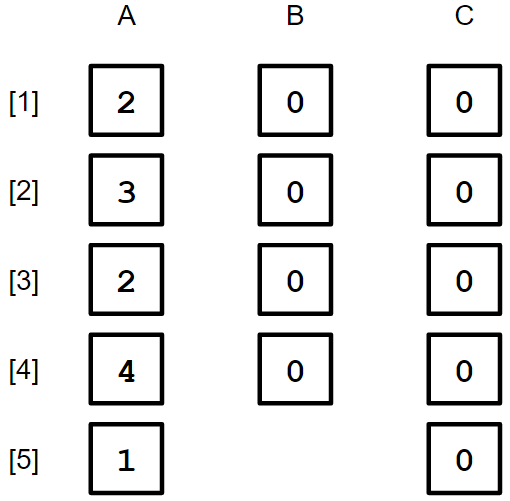
\includegraphics[width=1.2in]{_0000_count0.png} 
			\caption{Before sorting}
			\label{fig:count1}
		\end{subfigure}
		\begin{subfigure}{0.24\textwidth}
			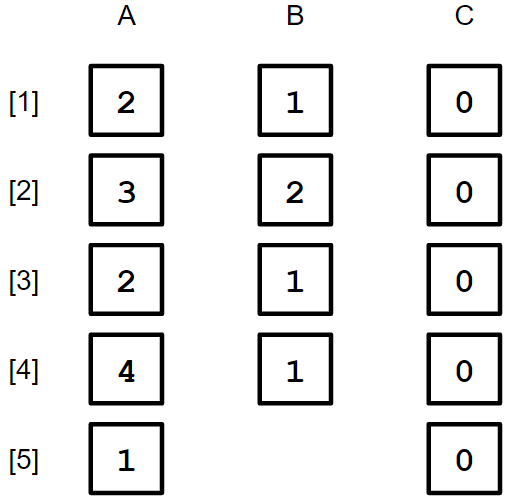
\includegraphics[width=1.2in]{_0002_count2.png}
			\caption{After 1st loop}
			\label{fig:count2}
		\end{subfigure}
		\begin{subfigure}{0.24\textwidth}
			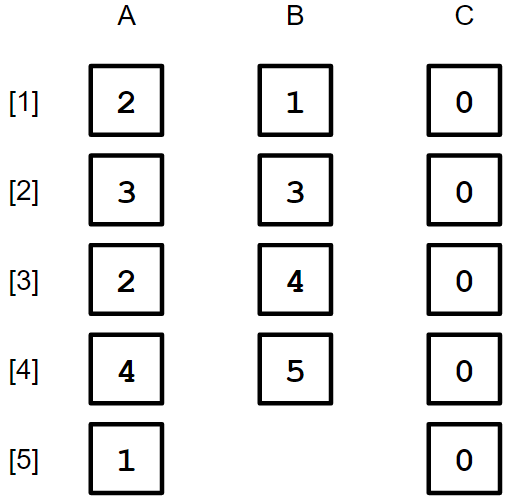
\includegraphics[width=1.2in]{_0001_count1.png}
			\caption{After 2nd loop}
			\label{fig:count3}
		\end{subfigure}
		\begin{subfigure}{0.24\textwidth}
			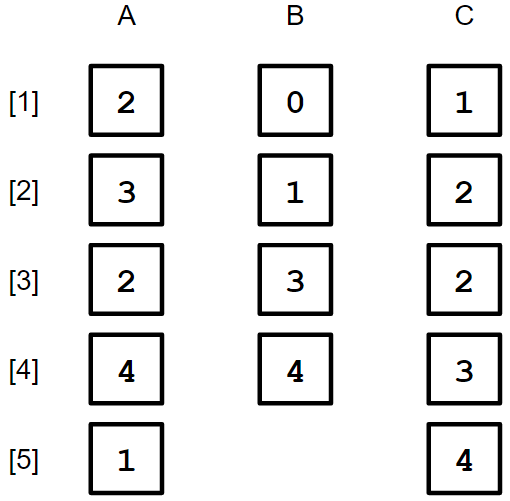
\includegraphics[width=1.2in]{_0003_count3.png}
			\caption{After 3rd loop}
			\label{fig:count4}
		\end{subfigure}

		\caption{Counting sort progression. The numbers on the left hand side denotes the index. The A column is the input array, B is the temporary working array, and C is the output.}
		\label{fig:countmerge}
	\end{figure}
	
	\subsection{Exploration of a New Sorting Algorithm}
	
	To fulfill the requirement of demonstrating original thought we looked at creating our own sorting algorithm.
	It proved difficult to come with a new sorting idea with so many existing sorting algorithm already on our mind.
	So instead we took a well known sorting algorithm, merge sort, and put a twist on it.
	The standard implementation of merge sort uses a recursive flow; each iteration calls the sort on itself and splits the list in two until it is completely divided.
	It then merges the smaller lists back together as it sorts\cite{wiki-mergesort}.
	A visual representation of this is shown in Figure~\ref{fig:stdmerge}.
	
	
\begin{figure}[H]
	
	\begin{subfigure}{0.49\textwidth}
		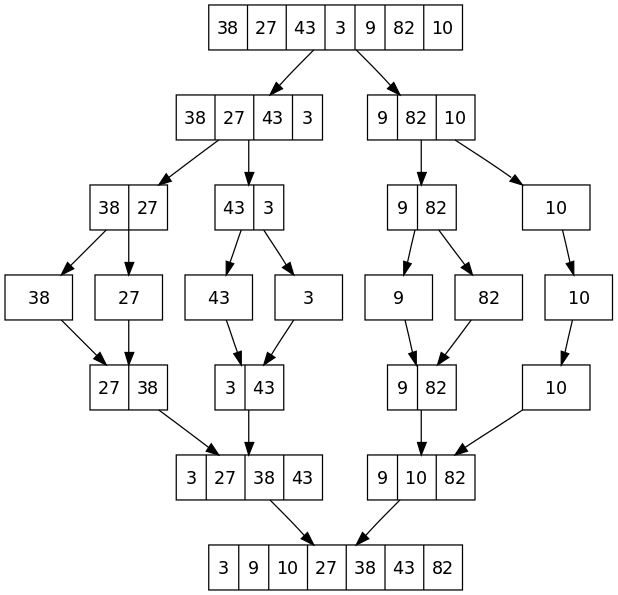
\includegraphics[width=2.5in]{Merge_sort_algorithm_diagram.png} 
		\caption{Standard Mergesort}
		\label{fig:stdmerge}
	\end{subfigure}
	\begin{subfigure}{0.49\textwidth}
		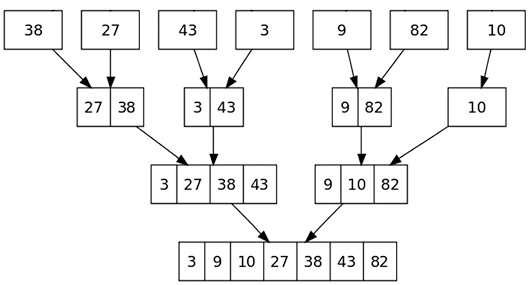
\includegraphics[width=2.5in]{New_merge_sort_algorithm_diagram.png}
		\caption{Our Mergesort}
		\label{fig:newmerge}
	\end{subfigure}
	
	\caption{Algorithm flow of the standard merge sort and our own implementation}
	\label{fig:bothmerge}
\end{figure}
	
	Now onto our variant.
	We decided to forgo the recursion and keep everything to one function call.
	The reasoning for this is, recursive functions have an overhead associated with them caused by the increased call stack \footnote{local variables must be reinitialized at each recursion level and the entrance of each function call must be stored so it can be returned to when the function exits}
	By skipping the recursion step it allows the algorithm to first start comparing pairs of elements.
	Visually it is represented by Figure~\ref{fig:newmerge}.
	Do not let the Figure~\ref{fig:newmerge} fool you however.
	Just because it looks like half the number of steps does not mean it is twice as fast.
	Before we go into the efficiency here is algorithm in its entirety is shown below in Snippet~\ref{snip:newmerge}.
	
	\begin{center}
		\captionof{Snippet}[New Mergesort]{Our own merge sort implementation that doesn't use recursion. Written in C++}
		\lstinputlisting{mergeSort2.cpp}
		\label{snip:newmerge}
	\end{center}

	Just knowing that an algorithm works is not enough\footnote{We do not prove that the new merge sort works, you must take our word that it does.}; an analysis of the runtime is also needed to ensure the algorithm performs as needed.
	The new merge sort algorithm was compared to a standard implementation of merge sort, introsort, quicksort, and insertion sort.
	To perform the tests, each algorithm was given the same randomly generated list starting with a size of 3 and doubling each time up to 12,582,912 elements.
	To our surprise the new merge sort outperformed many of the other algorithms.
	As shown in Figure~\ref{fig:algeff}, for lists with over 100 elements and up to the test limit the new merge sort performed 13X faster than the built in introsort and 3.6X faster than the standard merge sort.
	The efficiency of insertion sort on small list sizes can be seen in the graph as well.
	Quicksort is consistently faster than the new merge sort, with quicksort averaging 80\% of the runtime over the entire sample range.
	However, it can be seen that at around 2 million elements, the new merge sort pulled ahead.
	Each algorithm in Figure~\ref{fig:algeff} with the exception of insertion sort has an average runtime of $n \cdot log (n)$, yet it is clear from the plot that this approximation is not always precise enough when looking for the absolute fastest algorithm.

	\begin{figure}[H]
		\centering
		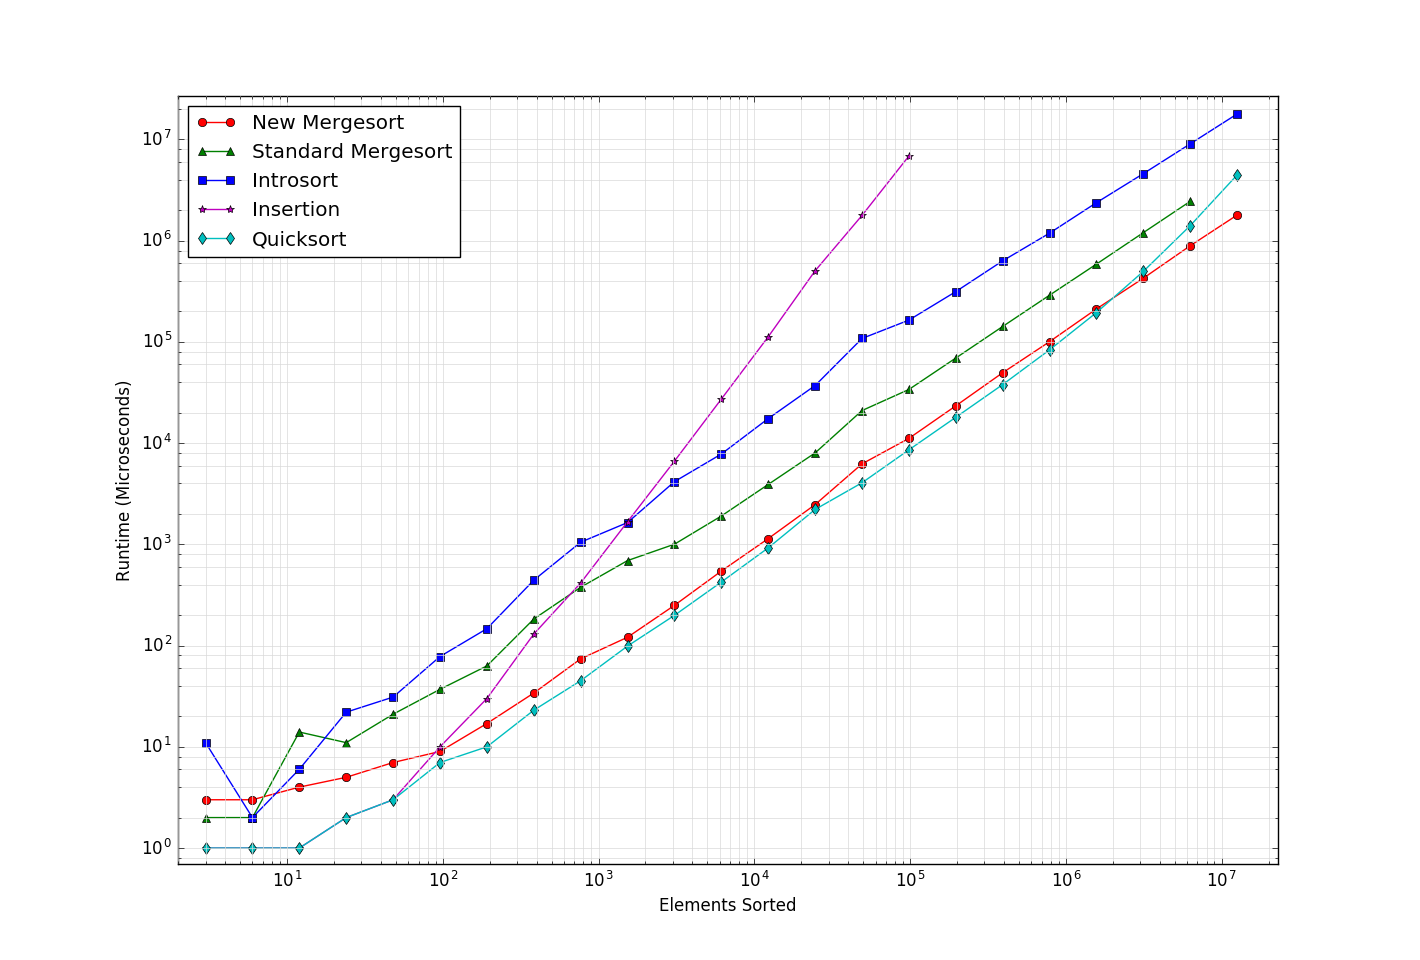
\includegraphics[width=6in]{figure_3.png}
		\caption{Algorithm Efficiency}
		\label{fig:algeff}
	\end{figure}
	
\section{Conclusion}

Sorting algorithms is an extensive subject and we were not able to cover it in its entirety, but compared to what students are exposed to in CS10 and CS11, this paper takes a huge step forward in explaining the intricacies of sorting algorithms.
For students moving along in the computer science, I hope they realize the importance in strategically choosing an algorithm for a given application. 
With sorting algorithms being a fundamental building block for countless other algorithms, choosing a strong foundation 



\pagebreak

\begin{thebibliography}{9}
	\bibitem{intro}
	Introduction to Algorithms, Third Edition,
	% todo: update author \emph{\LaTeX: a document preparation system},
	Thomas H. Cormen, Charles E. Leiserson, Ronald L. Rivest, Clifford Stein,
	2009.
	
	
	\bibitem{discrete}
	Discrete Mathematics with Applications, Fourth Edition,
	Susanna S. EPP,
	2010
	%todo cite at least once	
	
	
	\bibitem{wiki-callStack}
	Wikipedia: Call stack \url{https://en.wikipedia.org/wiki/Call_stack}
	
	\bibitem{wiki-recursiveFunction}
	Wikipedia: Recursive Function \url{https://en.wikipedia.org/wiki/Recursive_function}
	
	\bibitem{wiki-sortingAlgorithm}
	Wikipedia: Sorting Algorithm \url{https://en.wikipedia.org/wiki/Sorting_algorithm}
	
	\bibitem{wiki-mergesort}
	Wikipedia:~Merge Sort–~\url{https://en.wikipedia.org/wiki/Merge_sort}
		
\end{thebibliography}

\end{document}

